
\section{Diseño de la aplicación}

% Diagramas, explicación, etc. M.I.

La aplicación tiene la funcionalidad de recolectar publicaciones escritas en redes sociales que se refieren a un determinado programa de televisión, filtrar los datos relevantes, y usarlos para realizar mediciones sobre el programa en cuestión. 
Por otra parte, los mensajes son clasificados como positivos, negativos o neutrales por el módulo de Sentiment Analyisis.
\medskip

El diagrama de clases de esta aplicación está separado en varios gráficos para una mejor visualización. Para mostrar las relaciones entre clases que están en distintos gráficos, usamos como notación una ``caja'' particular para una de las clases en el gráfico donde aparece la otra, y señalamos la relación.

\subsection{Meters \& Views}

\begin{figure}[H]
\centering
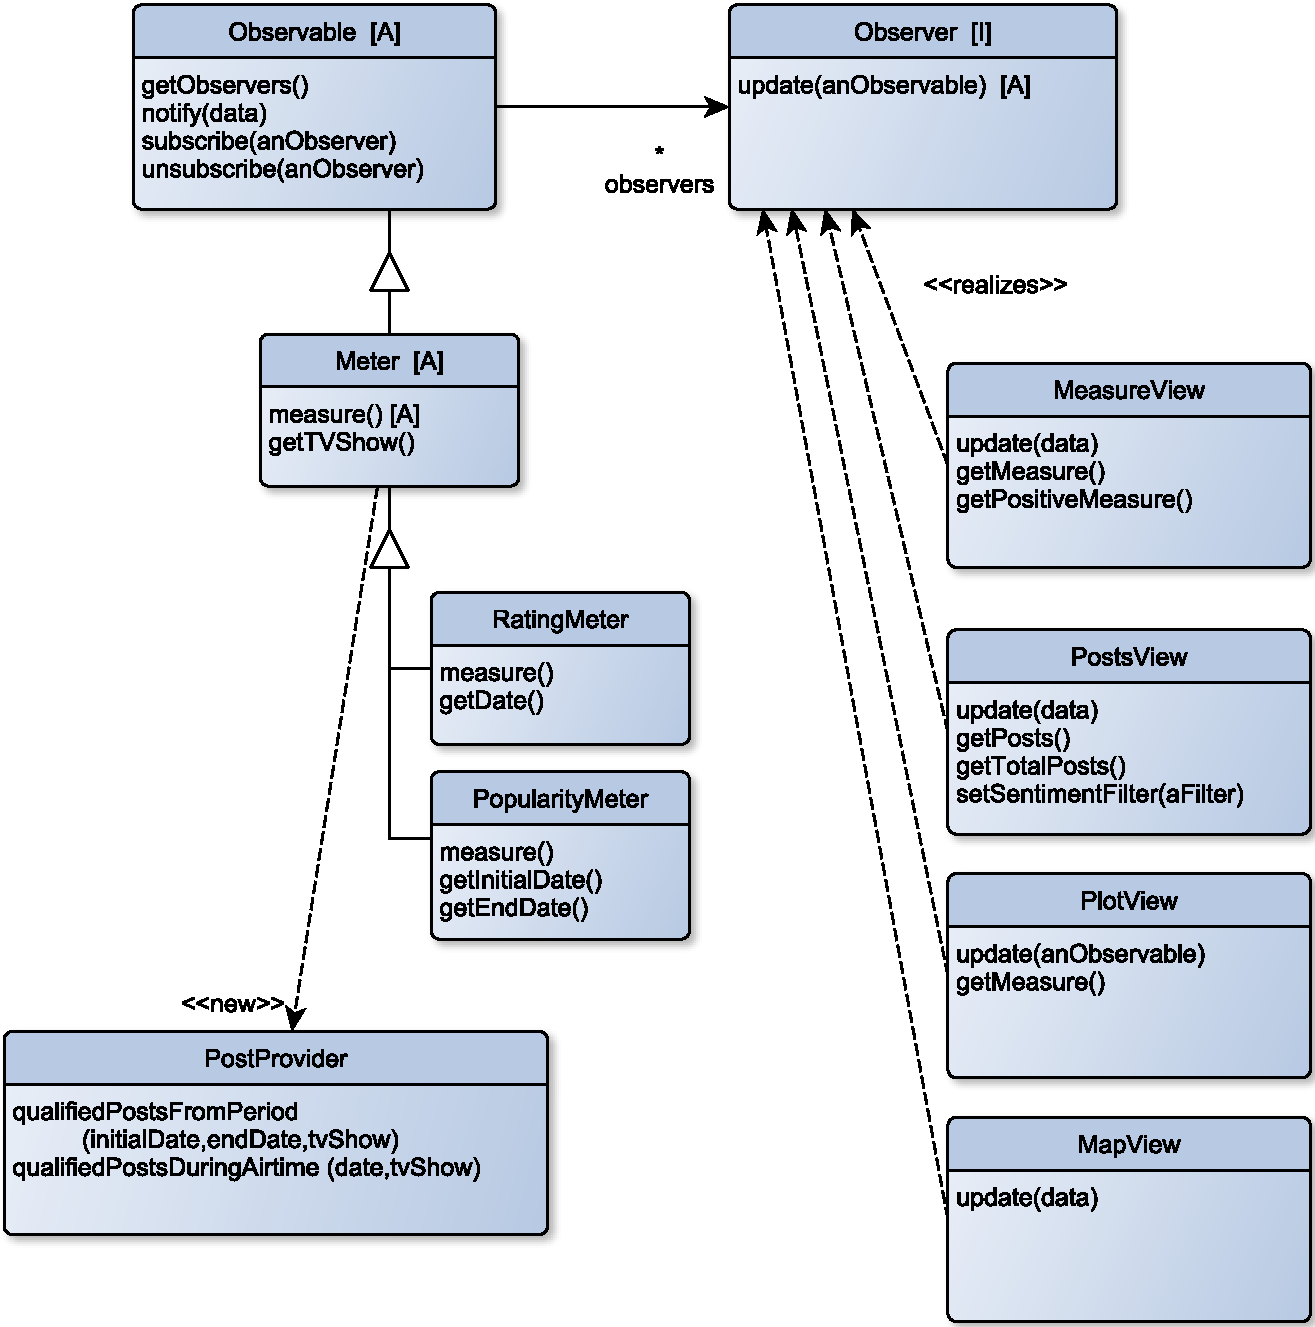
\includegraphics[width=0.8\textwidth]{graph/clase/meters.pdf}
\caption{Meters \& Views}
\end{figure}

Existen dos maneras de realizar mediciones en la aplicación: el rating y la popularidad. El rating consiste en una medición de la cantidad de posts recibidos para un programa en determinada fecha, durante el horario de emisión del programa, con un peso asignado según el sentimiento del mensaje. El rating puede consultarse ``en vivo'' para la fecha actual, mientras un programa se está emitiendo, y en ese caso se actualizará cada 10 segundos la información obtenida. La popularidad es una medición de la cantidad de posts de un programa, dado un intervalo de tiempo, en cualquier horario, también pesados según sentimiento.
\medskip

En la aplicación hay varias formas de visualizar esta información: la funcionalidad básica es la de mostrar un número que represente la medición de rating o popularidad (que aparece nombrada como MeasureView). Se puede pedir que el resultado se muestre en un gráfico (ver PlotView). También hay una funcionalidad para poder leer los mensajes concretos que la aplicación obtuvo y usó para sus cálculos (PostsView). Estos mensajes se muestran con autor, contenido y fecha, y se los puede filtrar de acuerdo a su sentimiento, en caso de que el usuario quiera ver u ocultar algún tipo de contenido. Por último está la opción de ver los posts en un mapa, donde se los clasifica por área geográfica y se muestra el valor de la medición para cada zona urbana principal (MapView).
\medskip

Cada una de estas vistas es independiente de las demás y trabaja con información que puede obtener del medidor que le corresponde. Esto permite que se puedan agregar o modificar los tipos de vista existentes sin un gran impacto en el resto de la aplicación, y además hace que no sea necesario mantener activas las vistas que el usuario no solicitó. Para lograr esto usamos el patrón de diseño \textit{Observer}, que nos permite desacoplar los objetos que conocen la información (los Meters) de los que reciben dicha información y la usan para generar una visualización particular (los Views).

\subsection{Posts \& Sentiment Analyisis}

\begin{figure}[H]
\centering
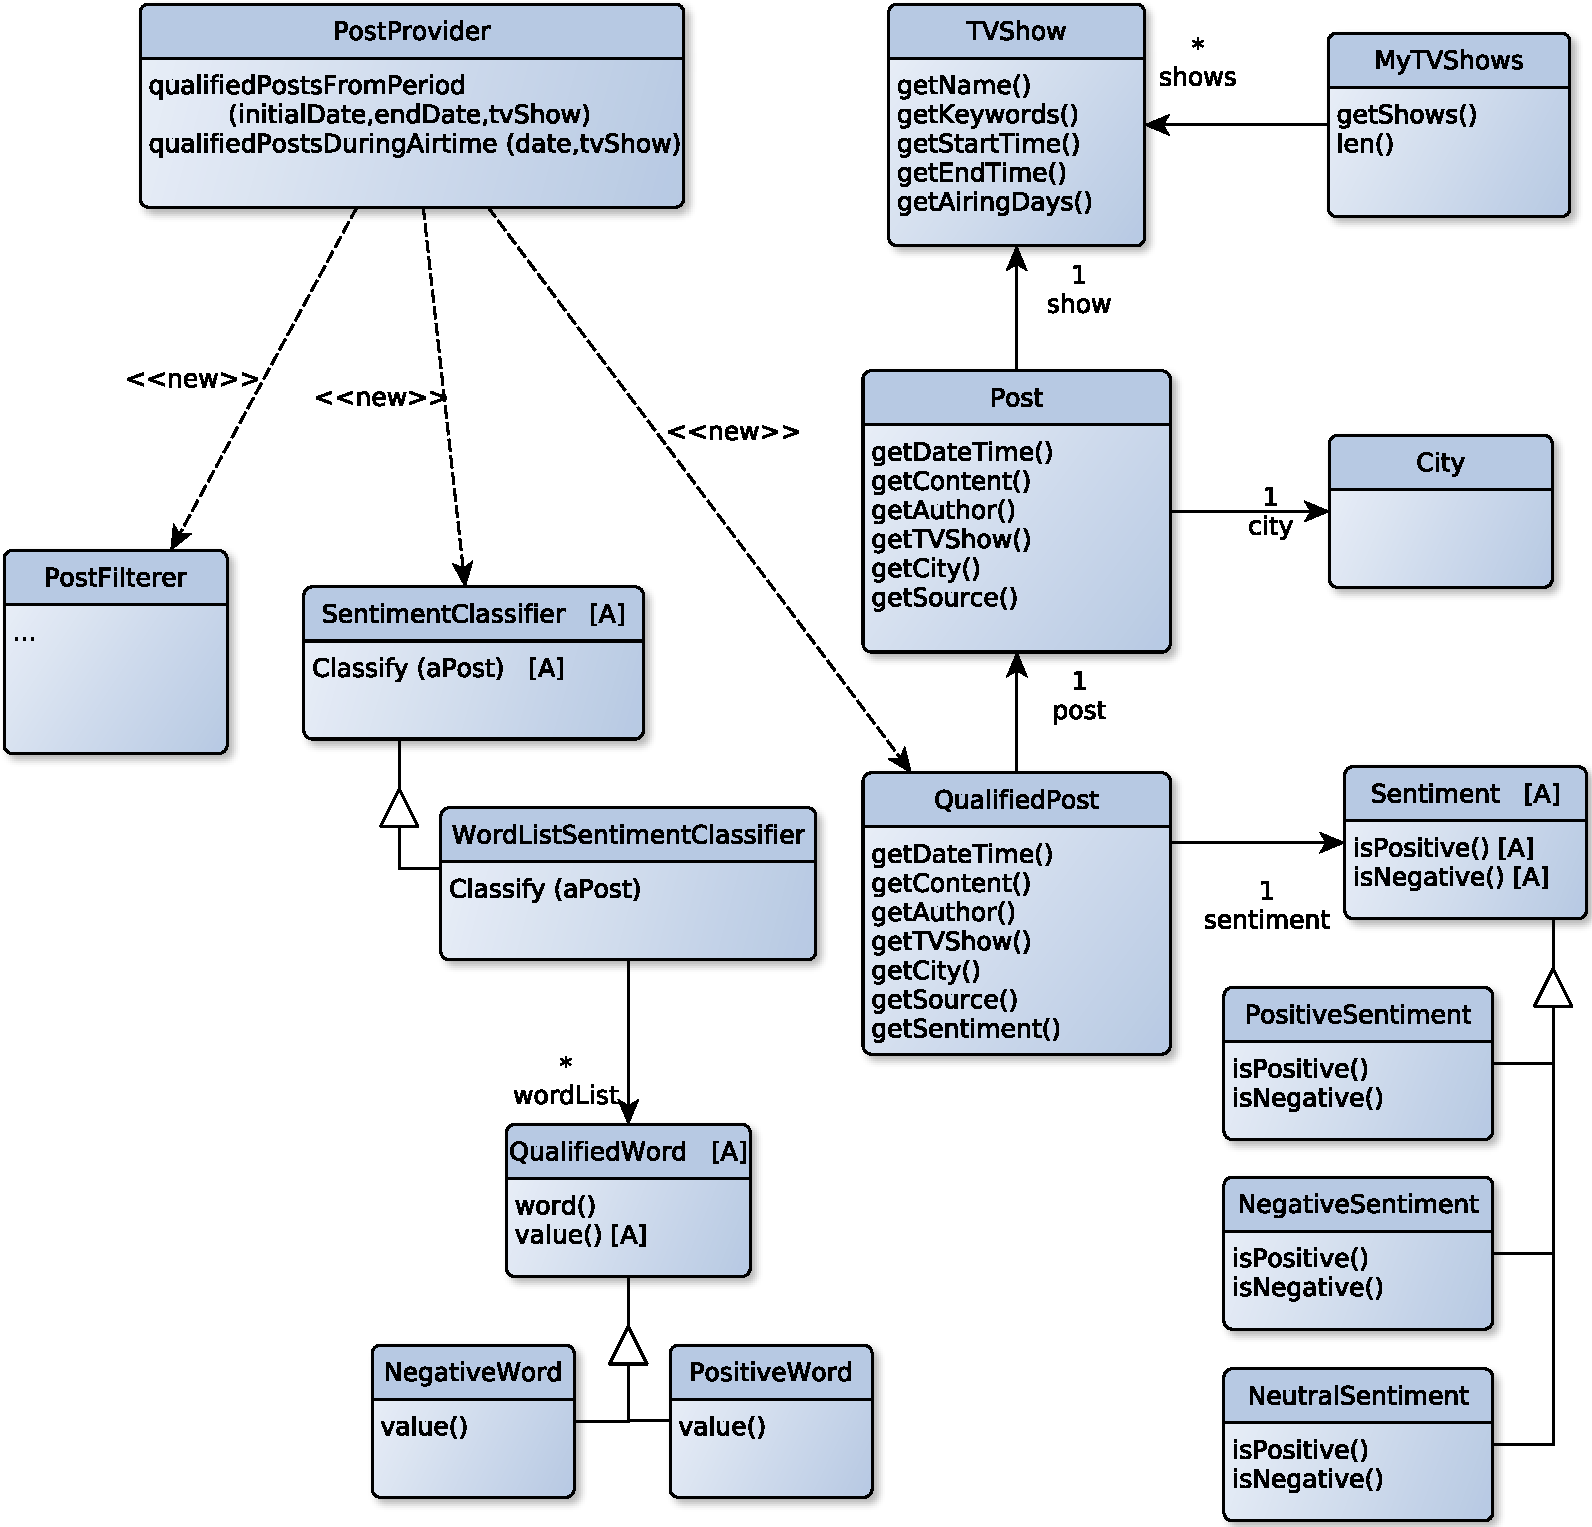
\includegraphics[width=\textwidth]{graph/clase/classifier.pdf}
\caption{Post Provider \& Sentiment Classifier}
\end{figure}

El \emph{post} es el elemento básico de esta aplicación, y consiste en un mensaje enviado a través de una red social. En principio es la representación de los datos de un \emph{tweet} que son útiles en nuestro programa, y también puede representar estos mismos datos, obtenidos de una red social distinta de \emph{Twitter}. Contiene algunos datos básicos como autor, texto del mensaje y fecha/hora de envío. También tiene un indicador de la ciudad desde la que se mandó el mensaje, en caso de que el autor haya activado la localización por GPS y de esa forma se pueda identificar su procedencia. Este indicador resulta útil para la vista de popularidad en mapa. Cada post también está vinculado con un único show de TV, el cual se le asigna basándose en palabras claves (generalmente \emph{hashtags}) contenidas en el mensaje. Por último, posee un indicador de sentimiento, que lo clasifica como positivo, negativo o neutro.
\medskip

El PostProvider es un objeto cuya función es la de obtener los posts necesarios para responder una consulta de rating o popularidad, y es invocado por los respectivos Meters para que consiga los posts específicos que se necesitan.
\medskip

El módulo de \emph{Sentiment Analyisis} consiste de un clasificador que asigna un valor a cada post y es llamado luego de recibir los datos de la red social e integrarlos al modelo de la aplicación. Existen tres valores para el sentimiento: positivo, negativo y neutro, y la manera de clasificar los posts es transparente al resto de las funcionalidades. En esta primera versión del programa, se usa un clasificador simple que lee de un corpus de palabras puntuadas como positivas o negativas, y realiza la clasificación según la cantidad de palabras de cada tipo que aparecen en cada mensaje. Se espera que a futuro se diseñe un nuevo clasificador con un criterio más complejo, y cuando esté implementado, se sustituya el que existe actualmente.


\subsection{Post Filterer}

\begin{figure}[H]
\centering
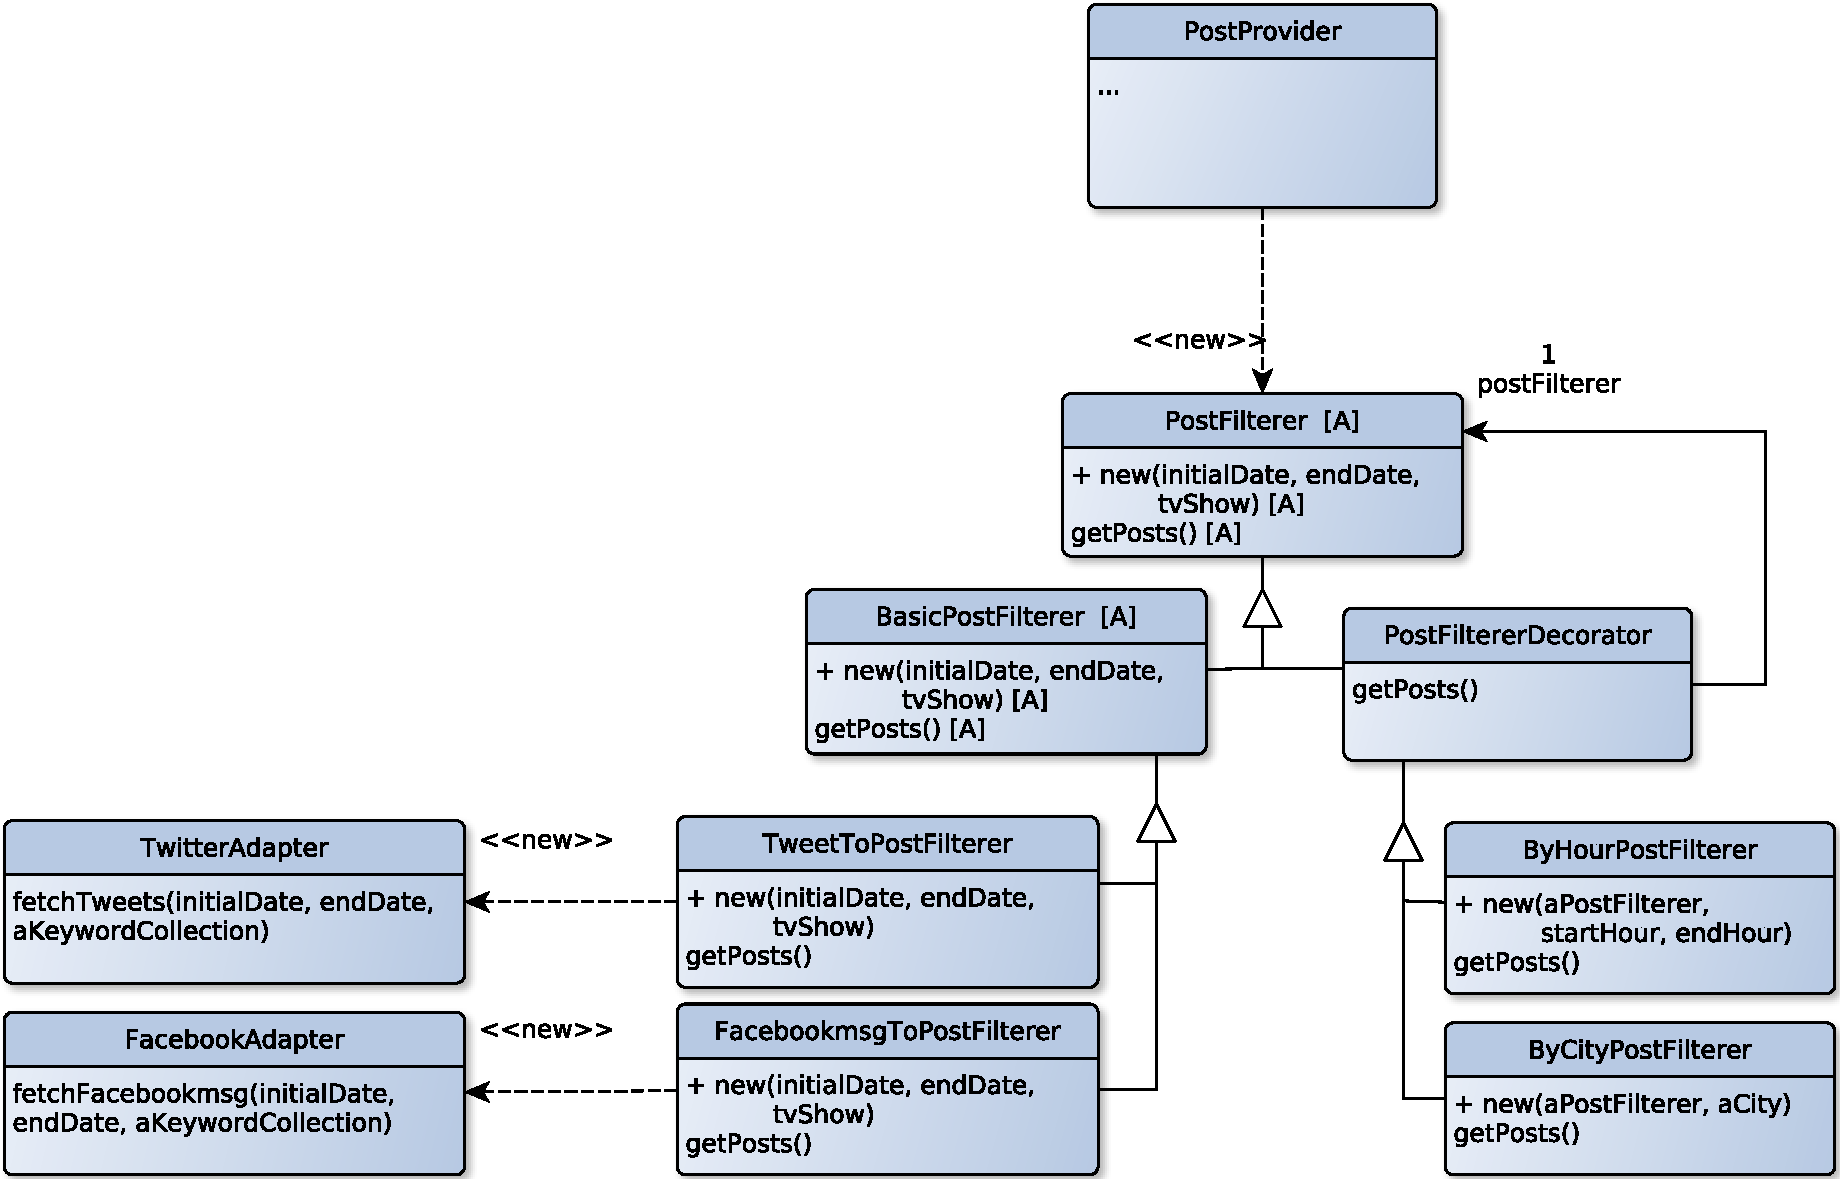
\includegraphics[width=\textwidth]{graph/clase/filterer.pdf}
\caption{Post Filterer}
\end{figure}



\subsection{Interfaz de usuario}

La interfaz de usuario es el elemento que coordina y da inicio al nivel más alto de la aplicación. Su responsabilidad es permitir que el usuario active las funcionalidades que desea usar, y eso lleve a crear los objetos necesarios. Cada vez que el usuario seleccione un programa de TV de la lista, y pida ver el rating o la popularidad de dicho programa para un intervalo, se creará un medidor correspondiente a los datos recibidos. De forma similar, cada vez que se seleccione una nueva manera de visualizar los datos, la interfaz pedirá la creación de una vista vinculada al medidor, para que muestre la información.

\subsection{Diagramas de secuencia y Objetos}

\begin{figure}[H]
\centering
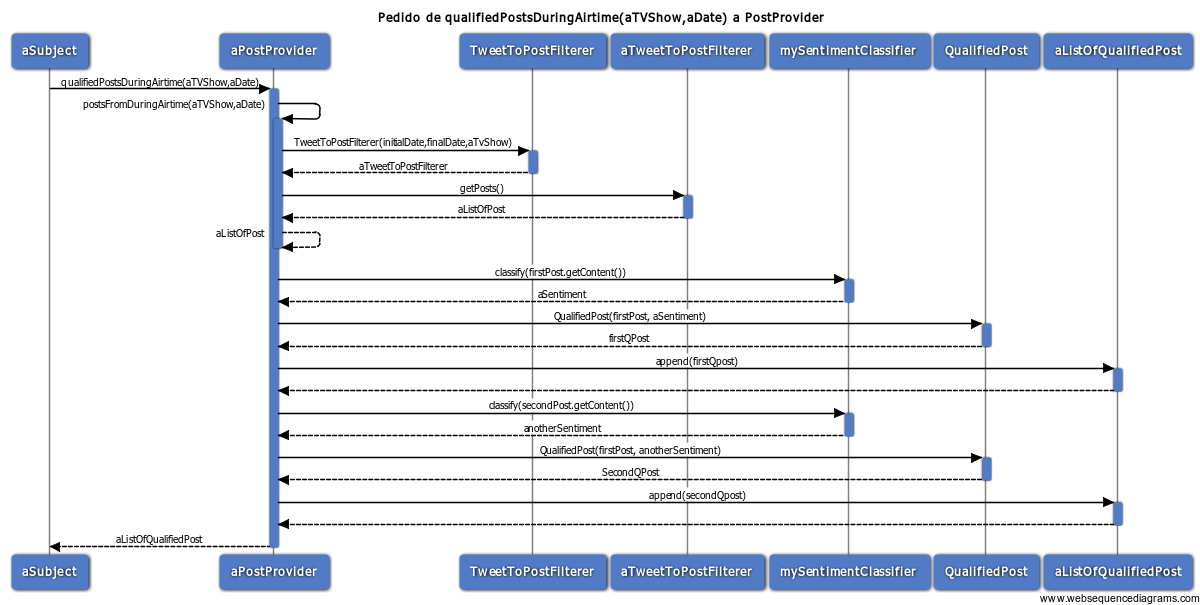
\includegraphics[width=\textwidth]{graph/diagramas_secuencia/PostProvider.png}
\caption{Post Provider}
\end{figure}

Aquí podemos observar como el sistema resuelve un pedido de rating para un determinado programa, cuales son los objetos que participan y cuales son creados. En concreto, llega un mensaje que tendrá como respuesta una lista de post calificados, por lo cual habrá que hacer lo siguiente: obtener la lista un lista de tweets para el programa en la hora de emisión (en el diagrama la comunicación con twitter no se muestra explicitamente), convertirlos a Post y darles un sentimiento.

\begin{figure}[H]
\centering
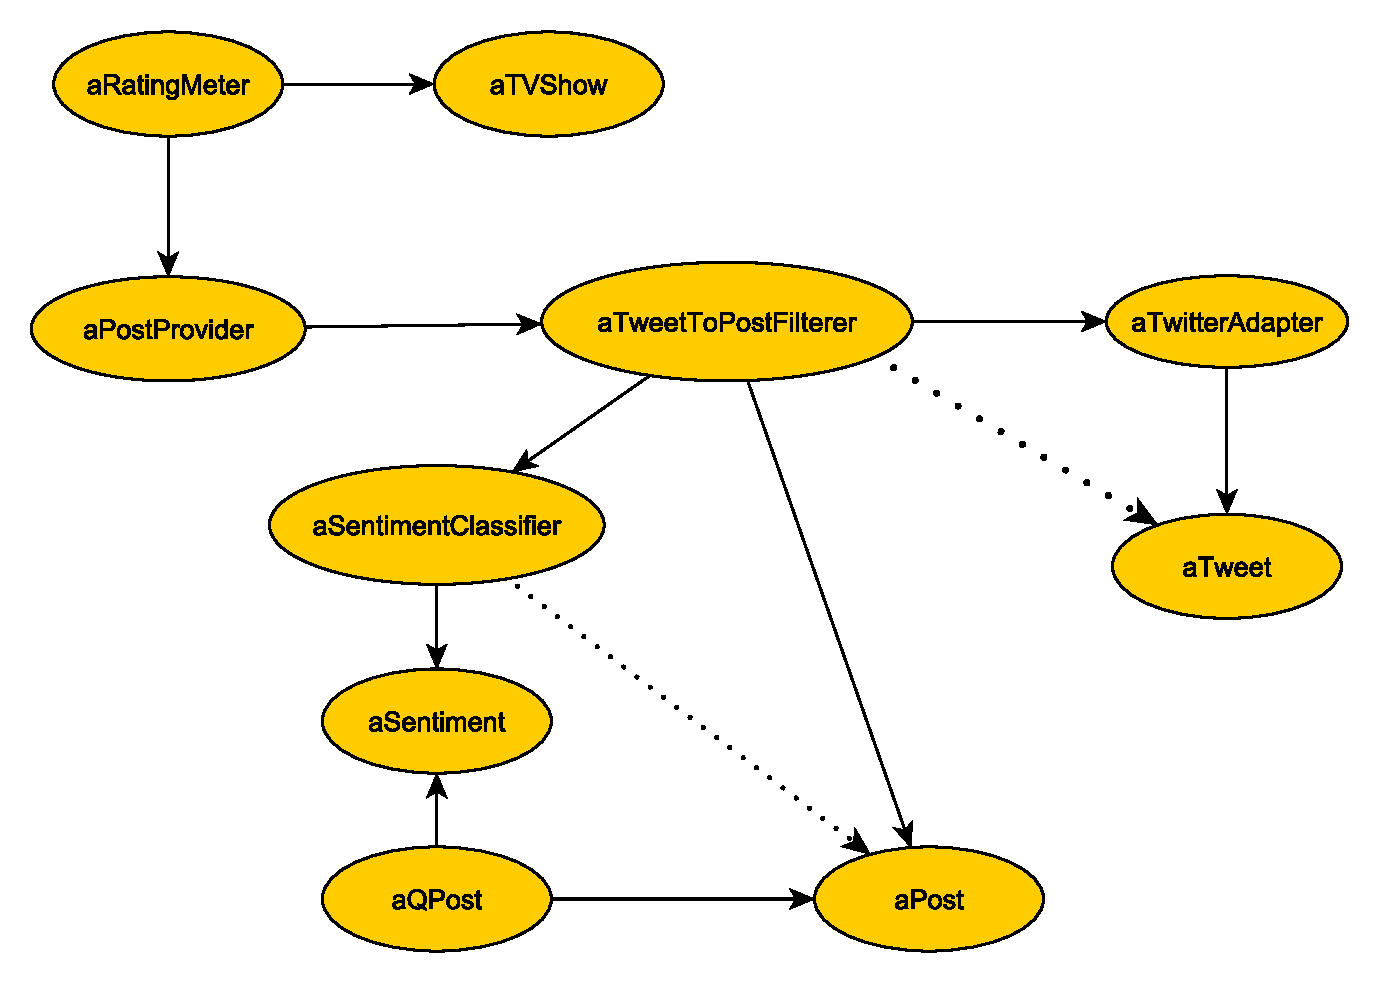
\includegraphics[width=\textwidth]{graph/objetos/PostProvider.pdf}
\caption{Post Provider (Objetos)}
\end{figure}



\begin{figure}[H]
\centering
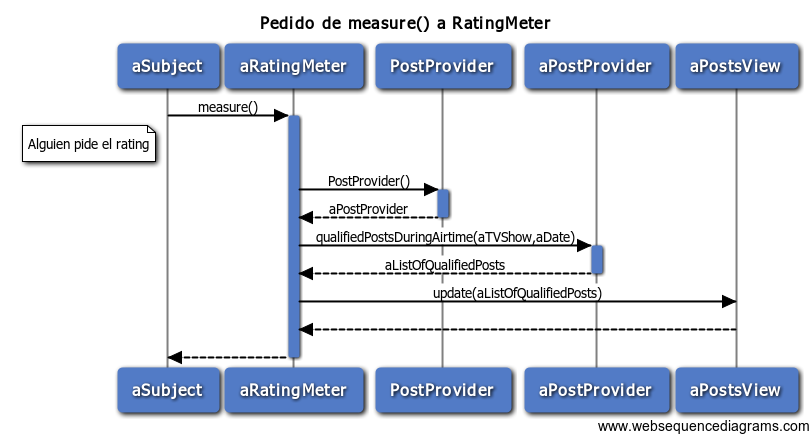
\includegraphics[scale=0.6]{graph/diagramas_secuencia/Rating.png}
\caption{Rating}
\end{figure}

Este diagrama representa el cálculo de la medición de rating. En está instancia, un objeto de RatingMeter ya ha sido creado, al igual que sus observadores quienes ya están subscriptos a alguno de sus eventos. Cuando es recibido el mensaje $measure()$ sea crea un Post Provider quien obtendrá los posts calificados. Luego se notificará a los observadores quienes, dependiendo de su funcionamiento, convertirán estos datos para ser utilizados por diferentes vistas.

\begin{figure}[H]
\centering
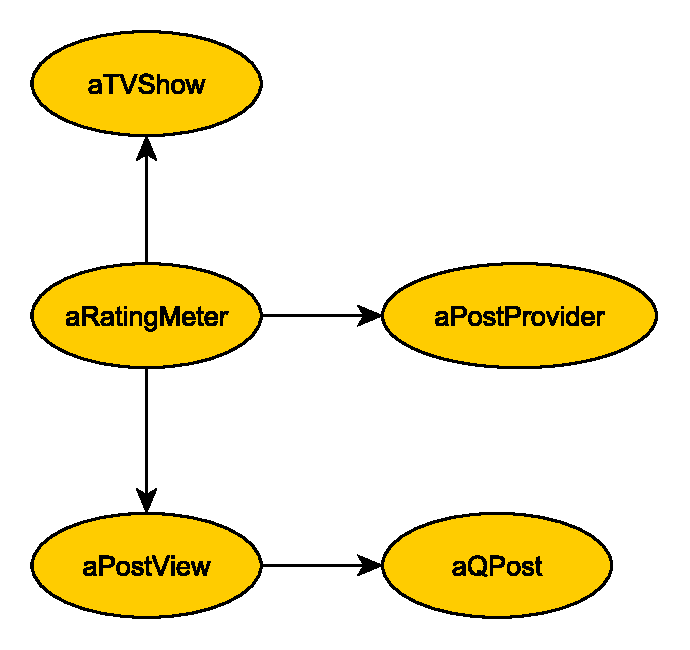
\includegraphics[scale=0.7]{graph/objetos/Rating.pdf}
\caption{Rating (Objetos)}
\end{figure}
